\documentclass{beamer}


% \setmainfont{XITS}

\usepackage[english]{babel}
\usepackage[UTF8]{ctex}              %lualatex用ctex
% \usepackage[utf8]{inputenc} 



%插入代码
\usepackage{listings}
\usepackage{fontspec}
\setmonofont{Monaco}
\usepackage{xcolor}

% Ah, that's good.
\usepackage{wasysym}

% \usepackage{geometry}
% \geometry{letterpaper}
% \usepackage{amssymb}
% \usepackage{wasysym}

\usepackage{graphicx} %插入图片的宏包
\usepackage{float} %设置图片浮动位置的宏包
\usepackage{subfigure} %插入多图时用子图显示的宏包

% 定义可能使用到的颜色
\definecolor{CPPLight}  {HTML} {686868}
\definecolor{CPPSteel}  {HTML} {888888}
\definecolor{CPPDark}   {HTML} {262626}
\definecolor{CPPBlue}   {HTML} {4172A3}
\definecolor{CPPGreen}  {HTML} {487818}
\definecolor{CPPBrown}  {HTML} {A07040}
\definecolor{CPPRed}    {HTML} {AD4D3A}
\definecolor{CPPViolet} {HTML} {7040A0}
\definecolor{CPPGray}  {HTML} {B8B8B8}
\lstset{
    columns=fixed,       
    frame=none,                                          % 不显示背景边框
    backgroundcolor=\color[RGB]{245,245,244},            % 设定背景颜色
    keywordstyle=\color[RGB]{40,40,255},                 % 设定关键字颜色
    numberstyle=\footnotesize\color{darkgray},           % 设定行号格式
    commentstyle=\it\color[RGB]{0,96,96},                % 设置代码注释的格式
    stringstyle=\rmfamily\slshape\color[RGB]{128,0,0},   % 设置字符串格式
    showstringspaces=false,                              % 不显示字符串中的空格
    language=c++,                                        % 设置语言
    morekeywords={alignas,continute,friend,register,true,alignof,decltype,goto,
    reinterpret_cast,try,asm,defult,if,return,typedef,auto,delete,inline,short,
    typeid,bool,do,int,signed,typename,break,double,long,sizeof,union,case,
    dynamic_cast,mutable,static,unsigned,catch,else,namespace,static_assert,using,
    char,enum,new,static_cast,virtual,char16_t,char32_t,explict,noexcept,struct,
    void,export,nullptr,switch,volatile,class,extern,operator,template,wchar_t,
    const,false,private,this,while,constexpr,float,protected,thread_local,
    const_cast,for,public,throw,std},
    emph={map,set,multimap,multiset,unordered_map,unordered_set,
    unordered_multiset,unordered_multimap,vector,string,list,deque,
    array,stack,forwared_list,iostream,memory,shared_ptr,unique_ptr,
    random,bitset,ostream,istream,cout,cin,endl,move,default_random_engine,
    uniform_int_distribution,iterator,algorithm,functional,bing,numeric,},
    emphstyle=\color{CPPViolet},
    basicstyle=\footnotesize\ttfamily,
}

%Theme
% customize your own color and navigation
\usetheme[RGB={12 72 66}]{Simple} % color
\useoutertheme{miniframes}              % navigation
% \usetheme{Berlin}
% \usecolortheme{beaver}
% \usepackage[english]{babel}
\usepackage{fancyhdr}        % header footer
\usepackage{graphicx}        % figure
\usepackage{algorithm2e}
\usepackage{booktabs}
\usepackage{xcolor}
\usepackage{bookmark}




\author{syh.hs}
\title{LUT-ICPC Day 2 树形结构、图论基础}
\date{\today}
\institute{兰州理工大学}

\AtBeginSection[]
{
  \begin{frame}
    \frametitle{Contents}
    \tableofcontents[currentsection]
  \end{frame}
}

\begin{document}
  % \maketitle

  % \tableofcontents
  

  % title
  % \frame[plain]{\titlepage}
  \begin{frame}[plain]
    \maketitle
    \begin{figure}[htbp] %H为当前位置,!htb为忽略美学标准,htbp为浮动图形
    \centering %图片居中
    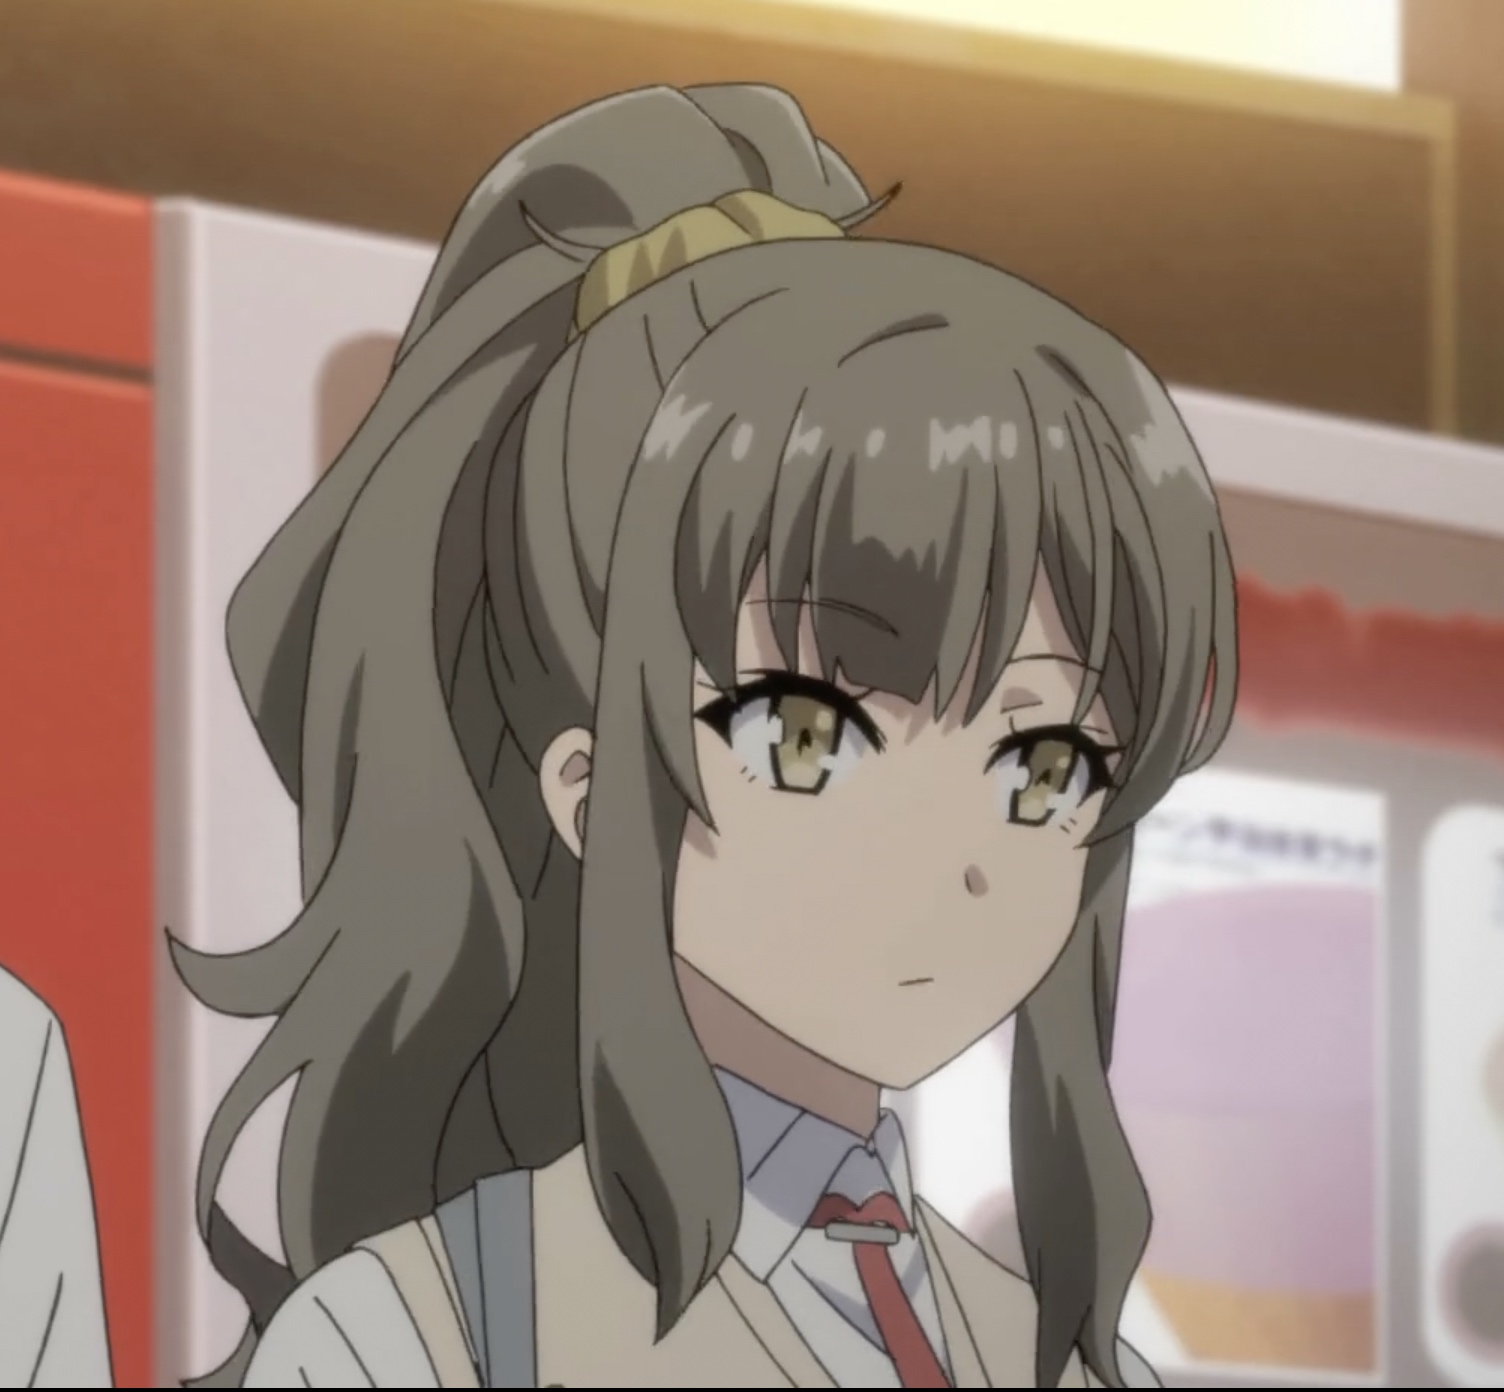
\includegraphics[width=0.3\textheight,height=0.2\textwidth]{new- 2.jpg} %插入图片,[]中设置图片大小,{}中是图片文件名
    % \caption{双叶天下第一可爱} %最终文档中希望显示的图片标题
    % \label{Fig.main2} %用于文内引用的标签
    \end{figure}
  \end{frame}

  \section{图论基础}

  \begin{frame}
    \frametitle{不严谨的定义}
    图论由点集和边集构成,其中点集非空

    \vspace*{1\baselineskip}
    
    边分为有向边和无向边

    \vspace*{1\baselineskip}
    
    \href{https://csacademy.com/app/graph_editor/}{一个好用的作图工具}
    
    \vspace*{1\baselineskip}

    度数表示与该节点关联的边数
    
    在有向图里对应的有\underline{入读}
    和\underline{出度}

    
  \end{frame}

  \begin{frame}
    \frametitle{不严谨的定义}
    自环
    
    重边

    补图,针对无向图

    反图,针对有向图

    菊花图,常用来卡解法

    简单路径

    连通|连通图|连通分量
  \end{frame}

  \begin{frame}{不严谨的定义}
    有根树|无根树

    父亲|祖先|子节点

    节点深度|树的高度

    完全二叉树|满二叉树

    前序|中序|后序 遍历
  \end{frame}

  \begin{frame}[fragile]
    \frametitle{存图}
    \begin{block}{直接存边}
      \begin{lstlisting}
struct Edge {
  int u, v, w;
  bool operator<(const Edge &a) const {
    return w<a.w;
  }
};
      \end{lstlisting}
    \end{block}

    \pause

    \begin{block}{邻接矩阵}
      不太用

      能直接排除重边的影响,别的没啥
    \end{block}
  \end{frame}

  \begin{frame}[fragile]
    \frametitle{存图}
      \begin{block}{邻接表}
        \begin{lstlisting}          
int n, m;
cin >> n >> m;
std::vector<std::vector<int>>adj(n + 1);
std::bitset<100010>vis; vis.reset();
for (int i=1; i<=m; i++) {
  int u, v; std::cin>>u>>v;
  adj[u].push_back(v);
}
function<void(int)> dfs=[&](int u)->void {
  vis[u]==1;
  for (auto it:adj[u]) if (vis[it]==0) dfs(dfs, it);
};
            \end{lstlisting}
      \end{block}
  \end{frame}

  \begin{frame}[fragile]
    \frametitle{存图}
      \begin{block}{链式前向星}
        \begin{lstlisting}
const int N=1e5+5;
const int M=1e6+5;
int tot, nxt[M], to[M], head[N];
void add(int u, int v) {
  to[++tot]=v, nxt[tot]=head[u], head[u]=tot;
}
int main() {
  int u;
  for (int i=head[u]; i; i=nxt[i]) {
    int y=to[i];
    /* code */
  }
  return 0;
}
        \end{lstlisting}
      \end{block}
  \end{frame}

  \begin{frame}
    \frametitle{存图}

    根据对应的情况来存图,例如用 Kruskal 找MST,则边要按权值排序,直接存边

    \vspace*{1\baselineskip}

    还有具体对应做法,对于树只存每个节点的父节点等等


  \end{frame}

  \begin{frame}
    \frametitle{遍历一个图}
    深度优先搜索(DFS):

    深搜树的时候先访问更深的节点,然后再访问同深度的节点,以此递归,对于图也是如此
    ,从源点开始,有访问的节点之后继续递归,然后回溯时访问同一级节点

    \vspace*{1\baselineskip}

    广搜(BFS)

    每个访问的点入队,出队的时候将所有能到的点入队

    -----------

    <- ....... <-

    -----------
    
  \end{frame}


  \begin{frame}[fragile]
    \frametitle{dfs序}
    正常dfs(深度优先搜索)遍历整个图

    每次访问一个新的节点,标记顺序

    以邻接表为例

    \begin{lstlisting}
vector<vector<int>> adj(n + 1);
vector<int> dfn(n + 1), vis(n + 1, 0);
function<void(int)> dfs = [&](int u) {
  static int dfc = 0;
  vis[u] = 1, dfn[u] = ++dfc;
  for (int v : adj[u])
    if (vis[v] == 0)
      dfs(v);
};
    \end{lstlisting}
  \end{frame}

  \begin{frame}[fragile]
    \frametitle{欧拉序}

    有两种形式

    形式1: 在深搜的过程中,出入各统计一次

      \begin{lstlisting}
vector<vector<int>> adj(n + 1);
vector<int> euler;
function<void(int,int)> dfs = [&](int u, int fa) {
  euler.push_back(u);
  for (int v : adj[u]) {
    if (fa == v) continue;
    dfs(v, u);
  }
  euler.push_back(u);
};
      \end{lstlisting}
  \end{frame}

  \begin{frame}[fragile]
    \frametitle{欧拉序列}
    \begin{figure}[!htb] %H为当前位置,!htb为忽略美学标准,htbp为浮动图形
      % \centering %图片居中
      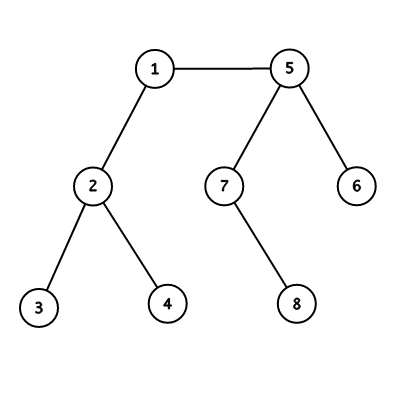
\includegraphics[width=0.5\textwidth,height=0.7\textheight]{euler_cnt.png} %插入图片,[]中设置图片大小,{}中是图片文件名
      % \caption{Main name 2} %最终文档中希望显示的图片标题
      % \label{Fig.main2} %用于文内引用的标签
    \end{figure}
  \end{frame}

  \begin{frame}
    \frametitle{欧拉序列}
    形式1:

    \vspace*{1\baselineskip}
    
    从1开始dfs的欧拉序就是 1 2 3 3 4 4 2 5 6 6 7 8 8 7 5 1 
    
    \vspace*{1\baselineskip}
    
    入加出减,前缀和维护,快速求子树的点权和
    
    \pause
    \vspace*{1\baselineskip}

    还有很多变形,自己可以操\mars 作
  \end{frame}

  \begin{frame}[fragile]
    \frametitle{欧拉序列}
    形式2:

    每经过一个点,就加入到序列中,回溯的过程也是

    \begin{lstlisting}
vector<int> dep(n + 1, 0), pre(n + 1, 0), suf(n + 1, 0);
vector<int> euler;

auto dfs = [&](auto self, int u, int fa, int _dep) {
  euler.push_back(u);
  pre[u] = euler.size() - 1;
  dep[u] = _dep;
  for (int v : adj[u]) {
    if (v == fa) continue;
    self(self, v, u, _dep + 1);
    euler.push_back(u); // 回来的时候还要经过
  }
  suf[u] = euler.size() - 1; // 返回时记录靠后的位置
};
    \end{lstlisting}
  \end{frame}

  \begin{frame}
    \frametitle{欧拉序列}
    按照上图的例子就是

    1 2 3 2 4 2 1 5 6 5 7 8 5 1

    \vspace*{1\baselineskip}

    共经过2n-1个点,因为经过了2(n-1)次边

    \vspace*{1\baselineskip}

    \pause

    之后会用到
  \end{frame}

  % \begin{frame}
  %   \frametitle{欧拉序列}
  %   \begin{figure}[H]
  %     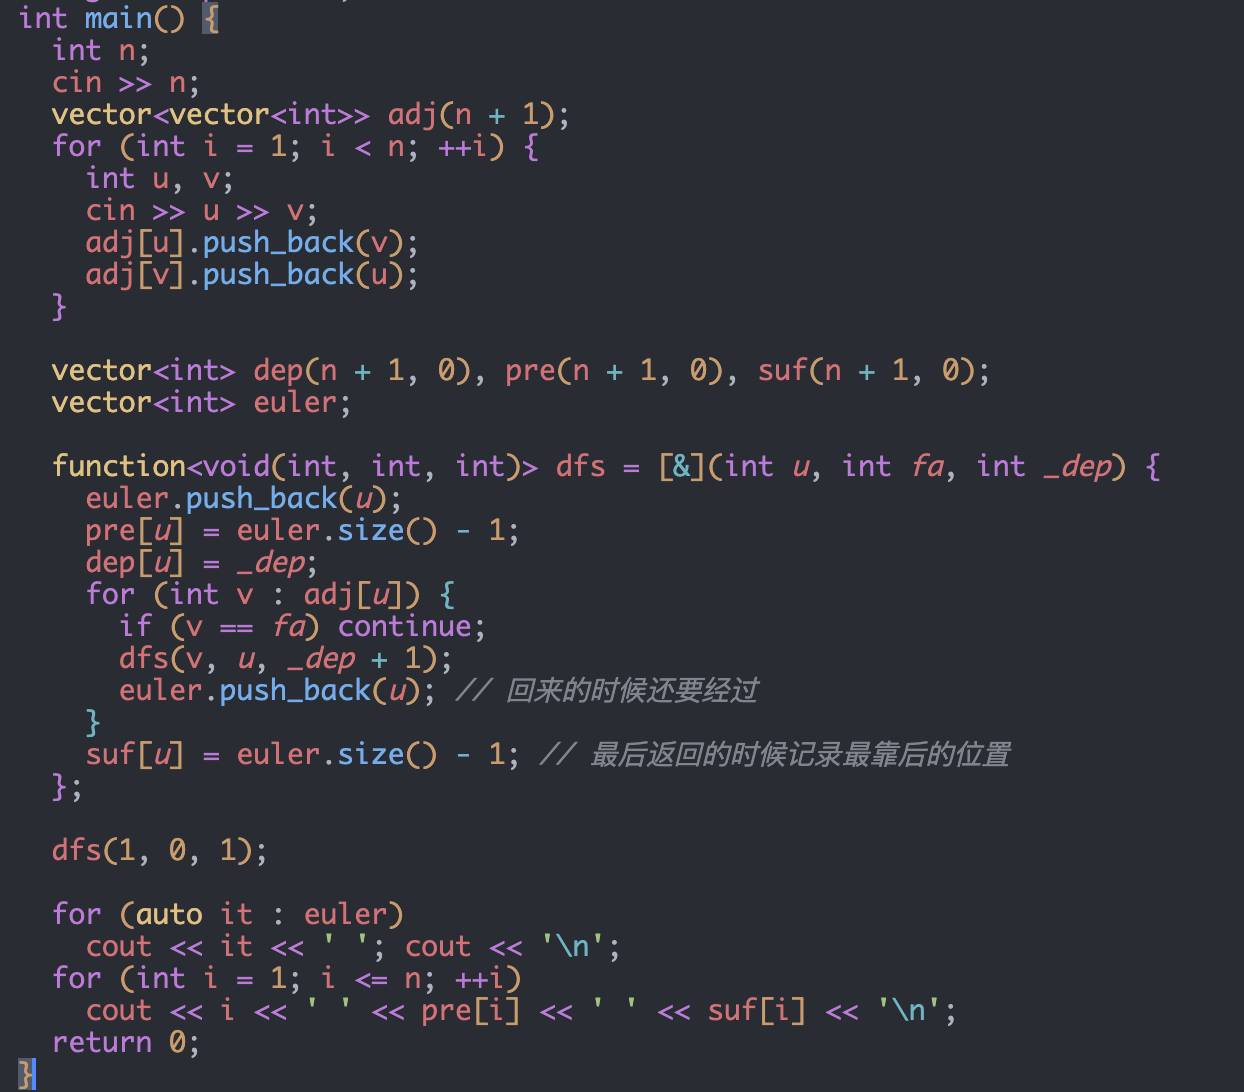
\includegraphics[width=0.9\textwidth,height=0.8\textheight]{day-p2.png}
  %   \end{figure}
  % \end{frame}

  \begin{frame}
    \frametitle{拓扑排序}
    \begin{block}{定义}
      拓扑排序要求对给定的一张图进行节点顺序排序,
      保证对于所有有向边(u,v),都有u的顺序在v的顺序之前
    \end{block}

    \pause
    
    \begin{block}{solution}
      动态维护一个入度为0的节点集合,这些就是当前能够排到顺序里的候选项
    \end{block}
    
    \pause

    至于字典序最大、最小那就是用什么维护的问题了

  \end{frame}

  \begin{frame}
    \frametitle{题目}
    \href{https://www.luogu.com.cn/problem/P1347}{洛谷 P1347 排序}

    \href{https://codeforces.com/gym/100801}{2015-2016 NEERC, Northern Subregional Contest G-Graph}
  \end{frame}

  \section{树上问题}

  \begin{frame}
    \frametitle{最近公共祖先 - LCA}
    \href{https://www.luogu.com.cn/problem/P3379}{模板题}

    \vspace*{1\baselineskip}
    
    给定一颗n个点的树,以及q个询问

    \vspace*{1\baselineskip}

    每个询问给定两个点(u,v),要求出深度最大的点,既是u的祖先,也是v的祖先,记为
    lca(u,v)
  \end{frame}

  \begin{frame}
    \frametitle{solution-倍增上跳}
      $\mathtt{dp[i][j]}$:$i$的 $2^j$ 祖先是谁

      \vspace*{1\baselineskip}
      
      $\mathtt{dp[i][j+1]=dp[dp[i][j]][j]}$
      
      \vspace*{1\baselineskip}
      
      利用倍增性质在($\mathtt{log_2}$高度)的时间内处理完
      
      \vspace*{1\baselineskip}
      
      求LCA就一起跳到同一个深度,然后再往上跳即可

      \vspace*{1\baselineskip}

      复杂度?
  \end{frame}

  \begin{frame}
    \frametitle{solution-欧拉序+RMQ}
    有欧拉序列之后,我们可以把树上问题转化成区间问题

    \vspace*{1\baselineskip}

    对于两个节点u,v,我们从 $\mathtt{min\{pos[u],pos[v]\}}$
    走到 $\mathtt{max\{pos[u],pos[v]\}}$ 的过程,不会经过深度比 LCA(u,v)更小的节点

    \pause
    \vspace*{1\baselineskip}
    
    那么就变成了区间求最小深度,把序列对应的深度数组维护出来,做RMQ,
    ST表可以解决这类静态问题

    \vspace*{1\baselineskip}

    \href{http://syh521.cn/file/lca-dfs-st.cpp}{代码}

    复杂度?
    
    \vspace*{1\baselineskip}

    还有四毛子,加减1 RMQ等特殊方法来做
  \end{frame}

  \begin{frame}
    \frametitle{Tarjan离线算法}
    离线?给出所有询问之后再输出答案也不迟

    \vspace*{1\baselineskip}
    
    我们存储了所有的询问,那么从底向上的考虑问题,假设当前在一个最小的子树,
    我们发现有一组询问$\mathtt{lca(u,v)}$,那么答案就是当前子树的根,
    处理完当前节点的所有子树之后,再往上走,依次处理涉及询问的点,
    答案始终是当前所在子树的根
    
    \vspace*{1\baselineskip}
    
    \href{http://syh521.cn/file/lca-tarjan.cpp}{代码}

    复杂度?
    
    \vspace*{1\baselineskip}
    
    对应的就有强制在线
  \end{frame}

  \begin{frame}
    \frametitle{CF191C}

    给定一颗树,有m次操作,每次操作给定(u,v),路径上的长度都加1

    \vspace*{1\baselineskip}

    最后输出边权
  \end{frame}

  \begin{frame}
    \frametitle{Solution}
    简单的树上差分+LCA

    \vspace*{1\baselineskip}

    把边权标在深度更大的点上,然后两端+1,lca-2,dfs从底向上做一遍前缀和即可
  \end{frame}

  \begin{frame}
    \frametitle{题目}

    \href{https://www.luogu.com.cn/problem/P3379}{模板}

    可以用树剖、LCT牛刀杀鸡

    \vspace*{1\baselineskip}
    
    \href{https://www.luogu.com.cn/problem/P2597}{[ZJOI2012]灾难}
    
    \vspace*{1\baselineskip}
    
    \href{https://codeforces.com/contest/1702/problem/G2}{CF805 G2}

    \vspace*{1\baselineskip}

    LCA的题还有很多,一般是结合别的操作,例如树上差分、DP
  \end{frame}

  \begin{frame}
    \frametitle{别的}
    其实还有很多内容,, 但是我怕讲不完了

    \vspace*{1\baselineskip}
    
    树的直径,直径数量,重心
    
    \vspace*{1\baselineskip}

    难一点、复杂一点像树剖、LCT这种,还是要靠自己去看..
  \end{frame}

  \section{最短路}

  \begin{frame}
    \frametitle{定义}
    \href{https://www.luogu.com.cn/problem/P3371}{P3371 【模板】单源最短路径(弱化版)}
    
    给定一个有向图,求出从某一点出发到所有点的最短路长度
  \end{frame}

  \begin{frame}
    \frametitle{Bellman-Ford}
    $\mathtt{dis[i]}$表示源点s到点i的最短距离,初值统一设置为$\infty$

    \vspace*{1\baselineskip}

    $\mathtt{dis[s]=0}$

    \vspace*{1\baselineskip}
    
    松弛操作: 对于存在的边$\mathtt{(u,v,w)}$有
    $\mathtt{dis[v]=min(dis[v],dis[u]+w)}$
    
    对于所有的边,松弛一遍的效果是什么?
    
    \pause
    \vspace*{1\baselineskip}
    
    从源点出发的所有最短路,边数+1,即新扩展了一个点
    
    \pause
    \vspace*{1\baselineskip}
    
    一条最短路最多有多少个点(最多松弛几轮)
  \end{frame}
  
  \begin{frame}
    \frametitle{负环}

    \href{https://www.luogu.com.cn/problem/P3385}{模板题}

    \vspace*{1\baselineskip}
    
    一条边权之和为负数的回路

    \vspace*{1\baselineskip}
    
    最多松弛n-1轮,如果第n轮还能松弛下去,说明图中存在一个负环
    
    \vspace*{1\baselineskip}
    
    \href{http://syh521.cn/file/Negative_ring.cpp}{代码}
  \end{frame}

  \begin{frame}
    \frametitle{SPFA}
    
    注意到只有一处的松弛成功之后,被松弛的点才会引起下一次松弛

    \vspace*{1\baselineskip}
    
    那么在松弛成功后,我们可以用队列维护被松弛的点,作为下一轮的候选项
    
    这就是队列优化的Bellman-Ford,还有别的很多优化方式..
    
    \vspace*{1\baselineskip}

    至于SPFA,早期国内选手习惯这么叫,对其中历史感兴趣的可以看这一篇
    \href{https://blog.csdn.net/sidnee/article/details/106231883}{博客}
  
  \end{frame}

  \begin{frame}
    \frametitle{SPFA}  

    注意到这样一来复杂度变得玄学,但是出题人很快就有了各种卡SPFA
    以及各类优化版本的\href{https://www.zhihu.com/question/292283275/answer/484871888}{手段}
    使其轻松达到$\mathtt{O(nm)}$
    
    \vspace*{1\baselineskip}
    
    卡掉一个普通SPFA并不难,只需要一个美丽的菊花图
    
    \vspace*{1\baselineskip}
    
    当然费用流的部分问题上SPFA还是好用的,只不过别在正权图求最短路用就是了
  \end{frame}

  \begin{frame}
    \frametitle{Dijkstra}
    节点分为两个集合
    
    一个是确定了最短路径的{$S$}和未确定的{$T$}

    初始化$\mathtt{dis(s)=0}$ 其余的dis均为$\infty$

    然后重复以下作直到$T$为空:

    1. 从{$T$}中,选取最距离源点最近的结点,移到{$S$}中
    
    2. 对刚刚加入{$S$}的结点的出边进行松弛
    
    \vspace*{1\baselineskip}
    
    照这个思路 暴力.. $\mathtt{O(N^2 + M) = O(N ^ 2)}$
    
    \vspace*{1\baselineskip}

    正确性可以自己尝试用反证法证明一下
  \end{frame}
  
  \begin{frame}
    \frametitle{Dijkstra}
    \begin{figure}
      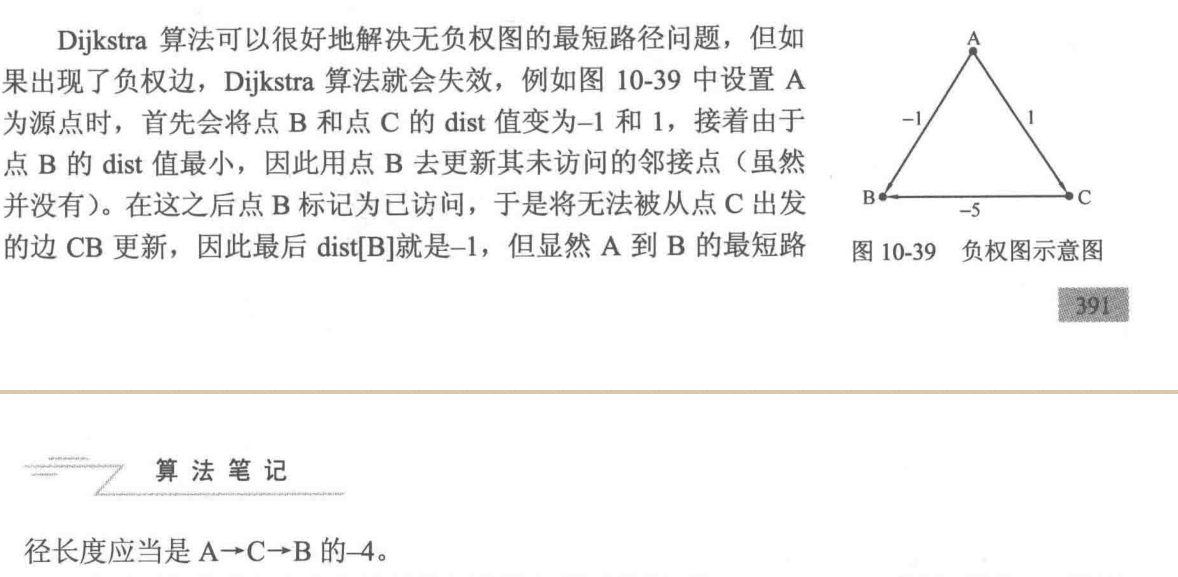
\includegraphics[width = \textwidth]{DijkstraCannot.png}
    \end{figure}
  \end{frame}

  \begin{frame}
    \frametitle{优化}
    \href{https://www.luogu.com.cn/problem/P4779}{P4779 【模板】单源最短路径(标准版)}

    慢的原因在第一步,怎么找到最近的节点

    \vspace*{1\baselineskip}
    
    用二叉堆优化,维护\{堆顶节点,边权\}的最小值,n次删除堆顶操作,
    m次插入(修改)操作,共 $\mathtt{O((n+m)logn)=O(MlogN)}$ 的复杂度
    
    \vspace*{1\baselineskip}
    
    STL的priority\_queue因为不能修改堆中的元素,也不能删除,规模在m,
    单次就是 $\mathtt{logM}$,总体就是 $\mathtt{O(MlogM)}$
    
    \vspace*{1\baselineskip}
    
    线段树的维护与手写堆类似,也是 $\mathtt{O(MlogN)}$
  \end{frame}

  \begin{frame}
    \frametitle{Floyd}

    用来求任意两个节点之间的最短路

    \vspace*{1\baselineskip}
    
    令$\mathtt{f[k][i][j]}$表示只经过$\mathtt{1\cdots k}$中的点,
    从i到j的最短路径

    \vspace*{1\baselineskip}
    
    显然$\mathtt{f[n][i][j]}$就是所求的答案数组,
    我们令$\mathtt{f[0][i][j]}$为邻接矩阵,显然有

    \vspace*{1\baselineskip}

    $\mathtt{f[k][i][j]=min\{f[k][i][j],f[k-1][i][k]+f[k-1][k][j]\}}$
  \end{frame}

  \begin{frame}[fragile]
    容易发现第一维是没有用的,每一层k都由k-1推导来,因此可以省略

    \vspace*{1\baselineskip}

    \begin{lstlisting}
for (k = 1; k <= n; k++)
  for (x = 1; x <= n; x++)
    for (y = 1; y <= n; y++)
      f[x][y] = min(f[x][y], f[x][k] + f[k][y]);
    \end{lstlisting}
  \end{frame}

  \begin{frame}
    \frametitle{Floyd}

    \begin{block}{找最小环}
      考虑环上最大的节点编号u
      
      枚举u,floyd的时候更新$\mathtt{\{f[u-1][x][y]+v(u,x)+v(u,y)\}}$最小值即可
    \end{block}

    \pause

    \begin{block}{传递闭包}
      求解一个图的任意两点是否连通

      \vspace*{1\baselineskip}

      把边权变成0/1,更新的时候改成或操作即可

      $\mathtt{f[i][j]|=f[i][k] \& f[k][j]}$
    \end{block}

    \pause

    如果出现$\mathtt{f[i][i]<0}$,那就说明出现了负环
  \end{frame}

  \section{生成树}

  \begin{frame}
    \frametitle{定义}
    一个连通无向图的生成子图,同时要求是树。

    即在图的边集中选择n-1条,将所有顶点连通。

    \vspace*{1\baselineskip}

    最小生成树 - MST 为边权和最小的生成树
  \end{frame}

  \begin{frame}
    \frametitle{Kruskal求最小生成树}
    将给定的边按照边权排序

    \vspace*{1\baselineskip}
    
    从小到大依次考虑每条边,如果边连接的两点不在一个集合内,那么加入这条边
    然后合并节点所在集合,直到插入n-1条边为止(或者集合大小为n),判断方式有很多..

    \vspace*{1\baselineskip}

    可以自己用数学归纳和反证法证明,考虑当前边的集合为F,下一条边是e,目标MST
    是T
  \end{frame}

  \begin{frame}
    \frametitle{Kruskal}
    反过来,一个正权图怎么找最大生成树?
  \end{frame}

  \begin{frame}
    \frametitle{Prim求最小生成树}
    每次选择一个最近的新的节点,收录到点集里,并用相关的边更新到别的点的距离

    证明同Kruskal
  \end{frame}

  \begin{frame}
    \frametitle{拓展}
    还有次小生成树,严格次小生成树等等

    \vspace*{1\baselineskip}

    这个可以用LCA、倍增等方式解决,自己看OI-wiki就好
  \end{frame}

  \begin{frame}
    \frametitle{Kruskal重构树}
    例题 \href{https://www.luogu.com.cn/problem/P1967}{货车运输}
    
    \vspace*{1\baselineskip}
    
    给定一个图,要求任意两点间所有路径最小权值的最大值
  \end{frame}

  \begin{frame}
    \frametitle{Solution - 最大生成树 + LCA}

    显然保存一个最大生成树,维护出来的最小值肯定最大,然后查询就好

    \vspace*{1\baselineskip}
    
    \href{http://syh521.cn/file/P1967.cpp}{代码}
  \end{frame}

  \begin{frame}
    \frametitle{Solution - kruskal 重构树}
    直接看图讲构造方式吧..

    \begin{figure}[htbp]
      \centering
      \begin{minipage}[t]{0.48\textwidth}
      \centering
      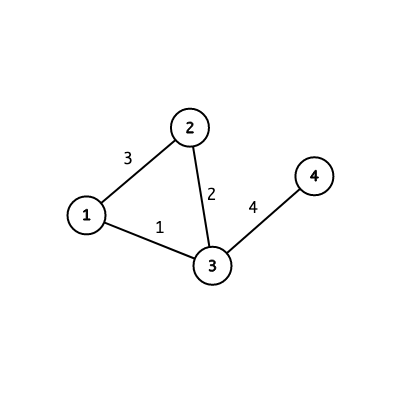
\includegraphics[width=6cm,height=6cm]{kruskal0.png}
      % \caption{World Map}
      \end{minipage}
      \begin{minipage}[t]{0.48\textwidth}
      \centering
      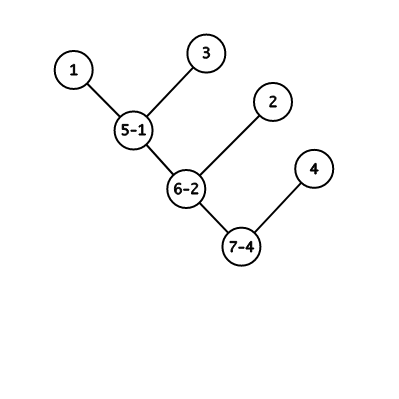
\includegraphics[width=6cm,height=6cm]{kruskal1.png}
      % \caption{Concrete and Constructions}
      \end{minipage}
    \end{figure}
  \end{frame}

  \section{连通性相关}

  \begin{frame}
    \frametitle{强连通}

    强连通分量 SCC - 极大强连通子图

    \vspace*{1\baselineskip}

    对于有向图G强连通,有任意两点都连通

    例如下图,SCC有三组 \{1,2,3\},\{4\},\{5\}

    \begin{figure}
      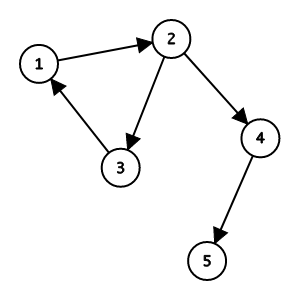
\includegraphics[width=0.4\textwidth,height=0.5\textheight]{scc_1.png}
    \end{figure}
  \end{frame}

  \begin{frame}
    \frametitle{Tarjan求SCC}
    \begin{block}{DFS生成树}
      搜索过程中将图的边分为四种

      1. 树边

      2. 返祖边 从dfn大的点指向dfn小的点

      3. 横叉边 指向一个dfn更小的点,但是不是祖先

      4. 前向边 遇到一个被访问过的子节点
    \end{block}
  \end{frame}

  \begin{frame}
    \begin{figure}
      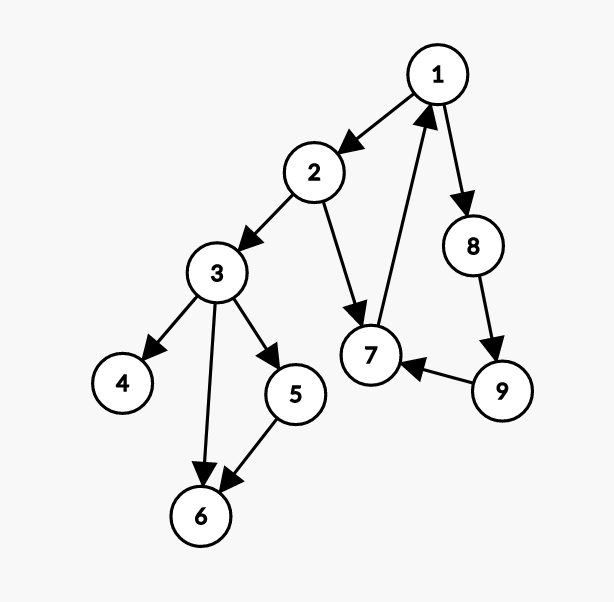
\includegraphics[width=0.4\textwidth,height=0.5\textheight]{scc_2.png}
    \end{figure}

    \pause
    
    如果u是某个强连通分量在搜索树中遇到的第一个节点,
    那么该SCC剩余节点都在以u为根结点的子树中
    
    \pause

    \vspace*{1\baselineskip}

    反证法证明?

  \end{frame}

  \begin{frame}
    \frametitle{Tarjan求SCC}
    维护两个东西

    $\mathtt{dfn_u}$ 这个很好理解

    $\mathtt{low_u}$: 设u为根的子树为$\mathtt{subtree_u}$,
    $\mathtt{low_u}$是以下节点的dfn最小值,$\mathtt{subtree_u}$中的节点,
    从 $\mathtt{subtree_u}$ 中节点通过一条非树边能到达的节点
    
    \vspace*{1\baselineskip}

    \pause

    感性理解:一个DAG(有向无环图)从任意节点都能往更深的地方走,如果这时候给它一条
    回到dfn更小的点的边,那么这个环里面的所有点构成一个SCC

    \pause

    \vspace*{1\baselineskip}

    一定构成吗?一定有环产生?

    \vspace*{1\baselineskip}

    如果有多条返回的边,自然是选择dfn最小的
  \end{frame}

  \begin{frame}
    \frametitle{Tarjan求SCC}
    dfs的时候通过一个栈,将节点都保存下来,在符合判定条件的时候,
    栈中节点构成一个SCC

    显然在SCC中只有一个点的$\mathtt{dfn_u=low_u}$

    \vspace*{1\baselineskip}
    
    对于节点u和它所有相邻的节点\{v\}

    1. v没有被访问,(u,v)是一条树边,那么就继续深搜,然后用$\mathtt{low_v}$
    更新$\mathtt{low_u}$

    2. v被访问过,并且在栈里面,那么就用 $\mathtt{dfn_v}$ 更新 $\mathtt{low_u}$

    3. v被访问过,并且不在栈里面,那么v所在的SCC已经被处理掉了,并且v也不能走到u,
    不然在1的时候就会继续深搜,一并处理掉

  \end{frame}

  \begin{frame}[fragile]
    \frametitle{Tarjan求SCC}
      \begin{lstlisting}
void tarjan(int u) {
  static int dfc = 0;
  low[u] = dfn[u] = ++dfc;
  sta.push(u);
  in[u] = 1;
  for (int &v : adj[u]) {
    if (!dfn[v]) {
      tarjan(v);
      low[u] = min(low[u], low[v]);
    } else if (in[v])
      low[u] = min(low[u], dfn[v]);
  }
  if (dfn[u] == low[u]) {
    // 栈顶所有元素弹出,直到u为止
  }
  // 弹出u,对应操作
}
      \end{lstlisting}
  \end{frame}

  \begin{frame}
    \frametitle{Kosaruju求SCC}
    对于一个图,如果正常的顺序有$\mathtt{A\to B}$,建立反图,也有
    $\mathtt{A\to B}$,不难发现原图上AB及其连边构成一个环

    \vspace*{1\baselineskip}
    
    后序遍历一个图,即左右根的方式,拿到序列之后反过来看,发现这个顺序满足拓扑序,称其为
    \textmd{逆后序}

    \pause

    \vspace*{1\baselineskip}
    
    顺序考虑逆后序的点,它和能到达的点构成一个SCC
    
    \pause
    \vspace*{1\baselineskip}

    思考一下横叉边,两端的点不在一个SCC内的情况,逆后序的顺序有影响吗?

    \href{http://syh521.cn/file/kosaraju.cpp}{代码}
  \end{frame}

  \begin{frame}
    \frametitle{割点}
    定义内容源自李煜东的WC课件

    \vspace*{1\baselineskip}
    
    在无向图G上定义:删掉某点P之后,G分裂为两个及两个以上的子图,则P为G的割点
    
    \vspace*{1\baselineskip}
    
    割点集合:无向连通图G中,如果有一个顶点集合,删除其中的点和关联的边之后,
    分裂为两个及以上的子图,则称该点为G的割点集合
    
    \vspace*{1\baselineskip}

    点连通度:最小的割点集合的大小-K,即删除任意K-1个点,图都连通
  \end{frame}

  \begin{frame}
    \frametitle{割边|BCC}

    定义类比割点

    \vspace*{1\baselineskip}
    
    双连通:点/边双连通图:(点/边)连通度大于1的图
    
    \vspace*{1\baselineskip}
    
    无向图的极大双连通子图称为双连通分量
  \end{frame}

  \begin{frame}
    \frametitle{求割点}
    Tarjan三件套的核心是什么?
    
    dfn与low数组,找到能回到的dfn最小的祖先

    \vspace*{1\baselineskip}

    \pause
    
    显然对于点u,tarjan过程中如果存在点v,通过边(u,v)以及递归得到
    $\mathtt{low_v\geq dfn_u}$,那么u就是一个割点

    \vspace*{1\baselineskip}
    
    \pause
    对于源点要特判..
    
    \pause
    \vspace*{1\baselineskip}

    对于点双连通 V-BCC,只要(u,v)满足了$\mathtt{low_v\geq dfn_u}$
    那么就依次取出栈中的点,和u构成一个点双连通分量

    \vspace*{1\baselineskip}

    当然割点u可能属于多个V-BCC,因此留在栈中,结束之后还剩一个V-BCC
  \end{frame}

  \begin{frame}
    \frametitle{找割边|边双连通}
    $\mathtt{tarjan}$的过程记录一个父节点fa,只要$\mathtt{low[v]>dfn[u]}$并且
    $\mathtt{low[u]=min(low[u],dfn[v])}$的时候$\mathtt{u!=fa[v]}$
    即可

    \vspace*{1\baselineskip}

    关键是验证是否只能通过树边回去
  \end{frame}

  \section{参考资料}

  \begin{frame}
    \frametitle{推荐阅读}

    \href{https://www.luogu.com.cn/blog/chengni5673/tu-lun-di-xiao-ji-qiao-yi-ji-kuo-zhan}{洛谷日报 - 图论的小技巧以及扩展}
  \end{frame}

  \begin{frame}
    \frametitle{参考资料}

    \href{https://oi-wiki.org/}{OI-wiki}

    \vspace*{1\baselineskip}
    
    图连通性若干拓展问题探讨-李煜东.pptx

    \vspace*{1\baselineskip}

    \href{https://www.zhihu.com/question/292283275/answer/484871888}{知乎问题}
  
  \end{frame}

\end{document}